\documentclass[12pt,a4paper]{article}
\usepackage[utf8]{inputenc}
\usepackage{float}
\usepackage[catalan]{babel}
\usepackage{graphicx}
\usepackage{geometry}
\usepackage{amsmath} 
\usepackage{url}
\usepackage{graphicx}     % Para insertar imágenes
\usepackage{hyperref}

\usepackage{fancyhdr}
\pagestyle{fancy}
\fancyhf{}
\rhead{
\includegraphics[height=1cm]{logoub.png}} % Right-aligned in header
\renewcommand{\headrulewidth}{0pt} % Remove header line

\geometry{margin=2.5cm}
\usepackage{amssymb} % Per utilitzar símbols matemàtics


\begin{document}

% Portada
\begin{titlepage}
    \centering
    \vspace*{1.5cm}
    
    {\Huge \textbf{Consum de Tapes als Locals Barcelonins} \par}
    \vspace{0.5cm}
    {\Large \textit{Entrega Teoria 1} \par}
    
    \vspace{2cm}
    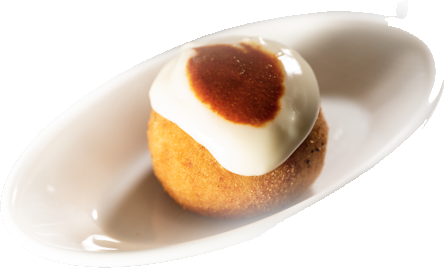
\includegraphics[width=0.8\linewidth]{Proyecto nuevo.png}
    
    \vfill
    {\large
    \textbf{Integrants del grup:} \\
    Pau Queralt Muñoz \\
    Alberto Moreno Marinez \\
    Gerard Fideu Garcia
    }
    
    \vspace{1cm}
    {\large Abril 2025 \par}
\end{titlepage}
% Índex
\tableofcontents
\newpage
\normalfont
\raggedright


\section{Introducció}

Amb el creixent auge dels brunchs i dels cafès d’especialitat, observem com es dilueix progressivament la cultura dels bars tradicionals que ofereixen menjar casolà i típic. Les tapes, un dels pilars fonamentals de la gastronomia barcelonina, sovint queden relegades a un segon pla davant de propostes més modernes i "instagrammables".

Com a grup d’amics apassionats per aquesta cultura, tenim el costum de relaxar-nos amb una bona tapa i un refresc en qualsevol bar autèntic de la ciutat. De fet, fa temps que compartim recomanacions, registrem quins bars ens agraden i fins i tot valorem les tapes que tastem (“Les bombes de la Cova Fumada són les millors: 9.75/10”).

A més, un dels membres del grup és celíac, fet que ens ha portat a tenir en compte les restriccions alimentàries a l’hora d’escollir locals: saber si ofereixen opcions sense gluten o plats aptes per a vegetarians és fonamental.

Aquest projecte neix, doncs, de tres motivacions principals:
\begin{itemize}
    \item \textbf{Preservar} i catalogar bars i tapes autèntiques de Barcelona abans que desapareguin.
    \item \textbf{Garantir} la seguretat alimentària de col·lectius amb restriccions (persones celíaques, vegetarianes, amb al·lèrgies, etc.).
    \item \textbf{Analitzar} patrons de consum: quines tapes són més populars? Hi ha estacionalitat? Quines combinacions o quantitats es repeteixen?
\end{itemize}
\section{Objectius}

L’elecció de les tapes com a eix temàtic per a la nostra base de dades respon a un conjunt d’objectius concrets que busquem assolir a través de la seva construcció i posterior explotació:

\begin{itemize}
    \item \textbf{Dissenyar i estructurar una base de dades relacional robusta}, que reculli informació rellevant sobre tapes i establiments de restauració barcelonins: ingredients, preus, opcions per a dietes especials, valoracions, zones i moments de consum.

    \item \textbf{Permetre consultes complexes mitjançant lògica relacional}, que ajudin a filtrar tapes segons criteris com el tipus d’ingredient, disponibilitat per a celíacs o vegetarians, barri, horari o preu mitjà.

    \item \textbf{Analitzar patrons de consum} a través de consultes SQL orientades a detectar quines tapes són les més demanades, quines combinacions apareixen amb més freqüència i si existeixen preferències estacionals o per franges horàries.

    \item \textbf{Estudiar les quantitats de consum i la seva variabilitat}, identificant establiments amb altes ràtios de comanda per client, o tapes que tenen més recurrència entre consumidors.

    \item \textbf{Proporcionar una eina útil per a la comunitat gastronòmica}, oferint una base de dades oberta que permeti tant a professionals com a aficionats localitzar tapes tradicionals, comparar establiments i prendre decisions de consum informades.

    \item \textbf{Preservar i donar visibilitat a la cultura gastronòmica local}, posant en valor les tapes clàssiques davant l’impacte creixent de tendències gastronòmiques globals i efímeres.
\end{itemize}
\section{Model Entitat-Relació}

A continuació, es mostren les entitats clau que conformen el nostre model entitat-relació, orientat a gestionar i analitzar informació sobre tapes i consum en bars de Barcelona.
\subsection{Entitats}
\subsubsection*{Bar}
\begin{itemize}
    \item \textbf{id\_bar (PK)}: Identificador únic del bar.
    \item \textbf{nom}: Nom comercial del bar.
    \item \textbf{direccio}: Adreça del local.
    \item \textbf{barri}: Zona o districte on es troba ubicat.
    \item \textbf{horari}: Horari d'obertura i tancament.
\end{itemize}

\subsubsection*{Tapa}
\begin{itemize}
    \item \textbf{id\_tapa (PK)}: Identificador únic de la tapa.
    \item \textbf{id\_bar (FK)}: Bar que serveix la tapa.
    \item \textbf{id\_consumicio (FK)}: Referència a la consumició on es demana.
    \item \textbf{nombre}: Nom de la tapa.
    \item \textbf{descripcio}: Breu descripció del plat.
    \item \textbf{preu\_base}: Preu base sense complements.
\end{itemize}

\subsubsection*{Ingredient}
\begin{itemize}
    \item \textbf{id\_ingredient (PK)}: Identificador únic de l'ingredient.
    \item \textbf{id\_tapa (FK)}: Tapa on apareix l’ingredient.
    \item \textbf{nom}: Nom de l’ingredient.
    \item \textbf{es\_alergen}: Booleà que indica si pot causar al·lèrgies.
\end{itemize}

\subsubsection*{Alergen}
\begin{itemize}
    \item \textbf{id\_alergen}: Identificador de l’al·lèrgen.
    \item \textbf{nom}: Nom de l’al·lèrgen (ex: gluten, ou).
    \item \textbf{efectes}: Breu explicació dels seus efectes.
\end{itemize}

\subsubsection*{Client}
\begin{itemize}
    \item \textbf{id\_cliente (PK)}: Identificador del client.
    \item \textbf{nom}: Nom del client.
    \item \textbf{mail}: Correu electrònic.
    \item \textbf{genere}: Gènere del client (si es registra).
    \item \textbf{es\_alergen}: Booleà per indicar si té alguna al·lèrgia.
\end{itemize}

\subsubsection*{Consumicio}
\begin{itemize}
    \item \textbf{id\_consumicio (PK)}: Identificador de la comanda o consumició.
    \item \textbf{id\_bar (FK)}: Bar on es fa la consumició.
    \item \textbf{id\_cliente (FK)}: Client que realitza la comanda.
    \item \textbf{preu\_total}: Import total de la consumició.
    \item \textbf{data\_hora}: Data i hora de la comanda.
    \item \textbf{nota}: Comentaris o puntuació.
\end{itemize}

\subsubsection*{InfoConsumicio}
\begin{itemize}
    \item \textbf{id\_consumicio (PK)}: Referència a la consumició.
    \item \textbf{id\_tapa (PK)}: Tapa que forma part de la comanda.
    \item \textbf{quantitat}: Quantitat d’unitats d’aquesta tapa en la consumició.
\end{itemize}
\subsection{Relacions i Cardinalitats}

\begin{itemize}
    \item \textbf{Bar \(\longleftrightarrow\) Tapa (1:N)} \\
    \textit{Explicació:} Un bar pot oferir moltes tapes diferents, però cada tapa està associada a un únic bar concret. Relació de "un a molts".
    
    \item \textbf{Bar \(\longleftrightarrow\) Consumicio (1:N)} \\
    \textit{Explicació:} Un bar pot registrar moltes consumicions fetes en el seu establiment. Cada consumició està vinculada a un únic bar. Relació de "un a molts".
    
    \item \textbf{Tapa \(\longleftrightarrow\) Ingredient (1:N)} \\
    \textit{Explicació:} Cada tapa pot contenir diversos ingredients, però un ingredient concret només pertany a una tapa en aquest model. Relació de "un a molts".
    
    \item \textbf{Ingredient \(\longleftrightarrow\) Alergen (N:M)} \\
    \textit{Explicació:} Un ingredient pot contenir diversos al·lèrgens (ex: ou i gluten), i un al·lèrgens pot aparèixer en múltiples ingredients. Relació de "molts a molts".
    
    \item \textbf{Client \(\longleftrightarrow\) Alergen (N:M)} \\
    \textit{Explicació:} Un client pot ser al·lèrgic a diversos al·lèrgens, i un al·lèrgens pot afectar múltiples clients. Relació de "molts a molts".
    
    \item \textbf{Client \(\longleftrightarrow\) Consumicio (1:N)} \\
    \textit{Explicació:} Un client pot fer diverses consumicions al llarg del temps, però cada consumició està associada a un sol client. Relació de "un a molts".
    
    \item \textbf{Consumicio \(\longleftrightarrow\) InfoConsumicio (1:N)} \\
    \textit{Explicació:} Una consumició pot incloure diverses tapes (amb quantitats diferents), però cada entrada d’InfoConsumicio està vinculada a una sola consumició. Relació de "un a molts".
    
    \item \textbf{InfoConsumicio \(\longleftrightarrow\) Tapa (N:1)} \\
    \textit{Explicació:} Una entrada d’InfoConsumicio fa referència a una única tapa, però una mateixa tapa pot aparèixer en moltes consumicions. Relació de "molts a un".
\end{itemize}
\subsection{Model E-R:}

A continuació es mostren els diagrames dels nostres models Entitat-Relació, un primer prototip que vam fer a paper, i un model polit en PlantUML que permet la modificació i ampliació senzilla del model.

\begin{figure}[ht]
    \centering
    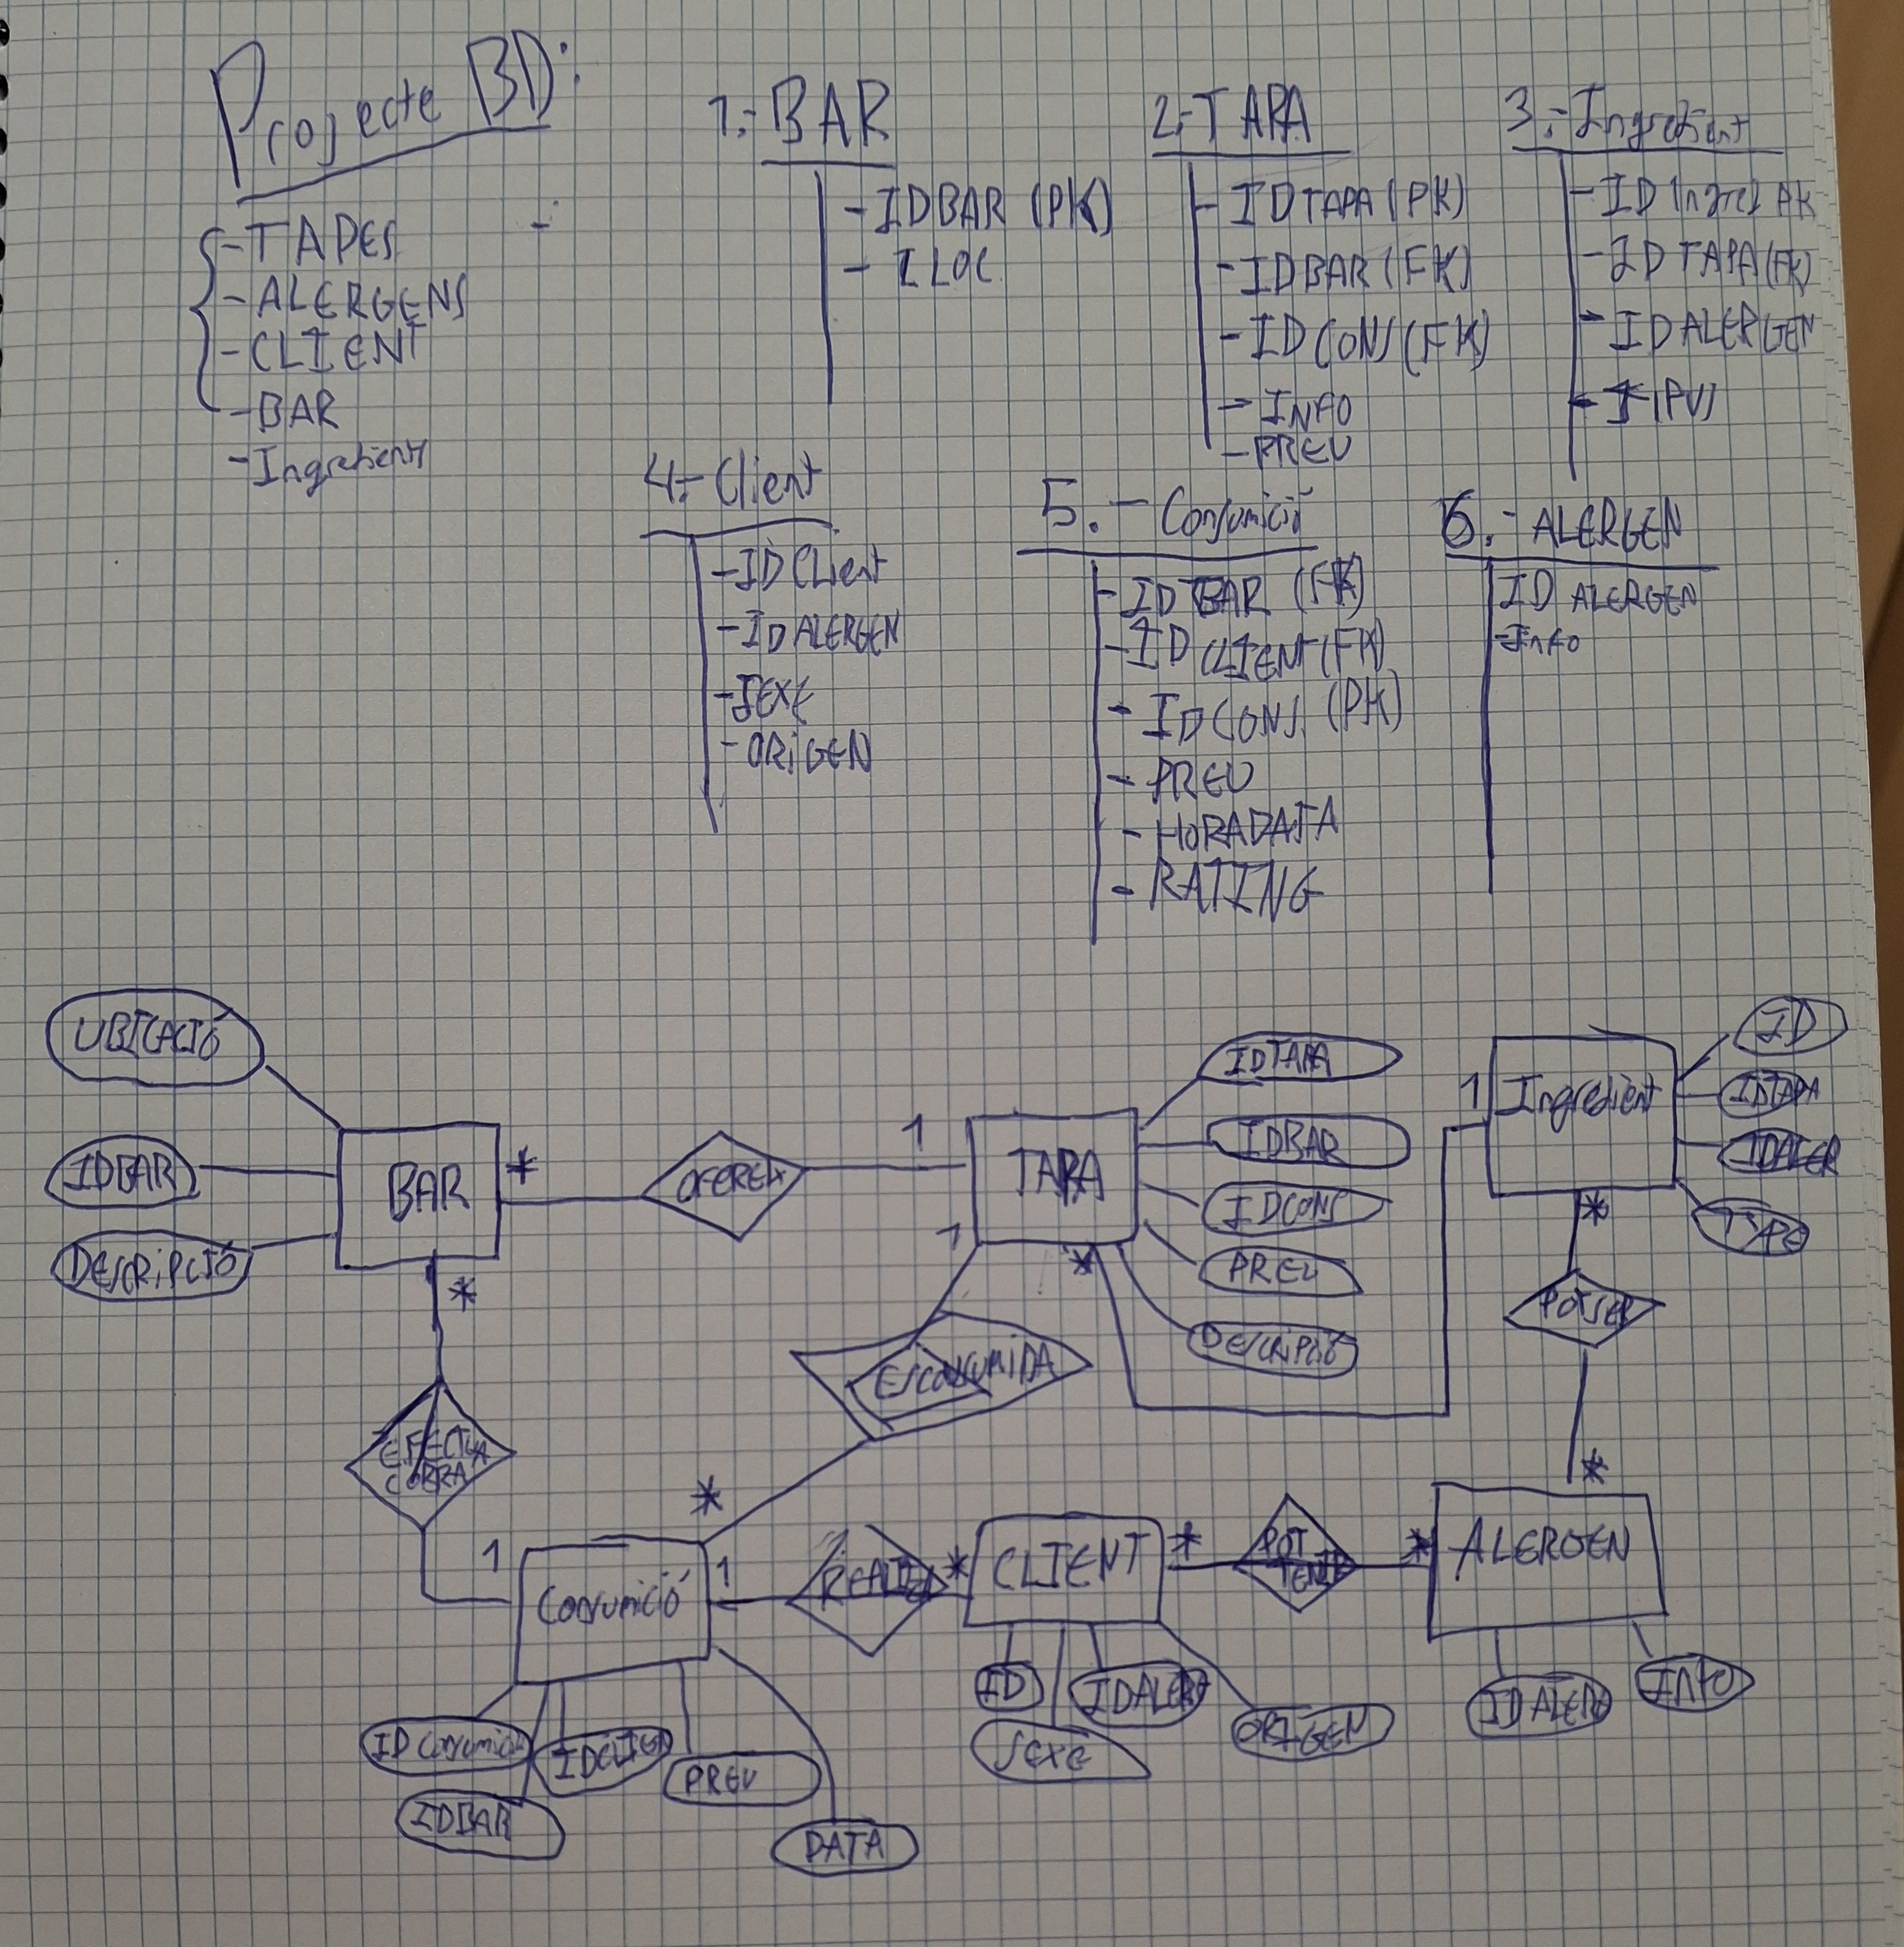
\includegraphics[width=0.5\linewidth]{diddy.jpg}
    \caption{Prototip-ER-1 a paper}
    \label{fig:enter-label}
\end{figure}

El següent diagrama mostra el model Entitat-Relació generat amb PlantUML, on es detallen les entitats clau del nostre sistema i les seves relacions. Aquest model és l'evolució del prototip inicial i està dissenyat per facilitar futures modificacions.

\begin{figure}[H]
    \centering
    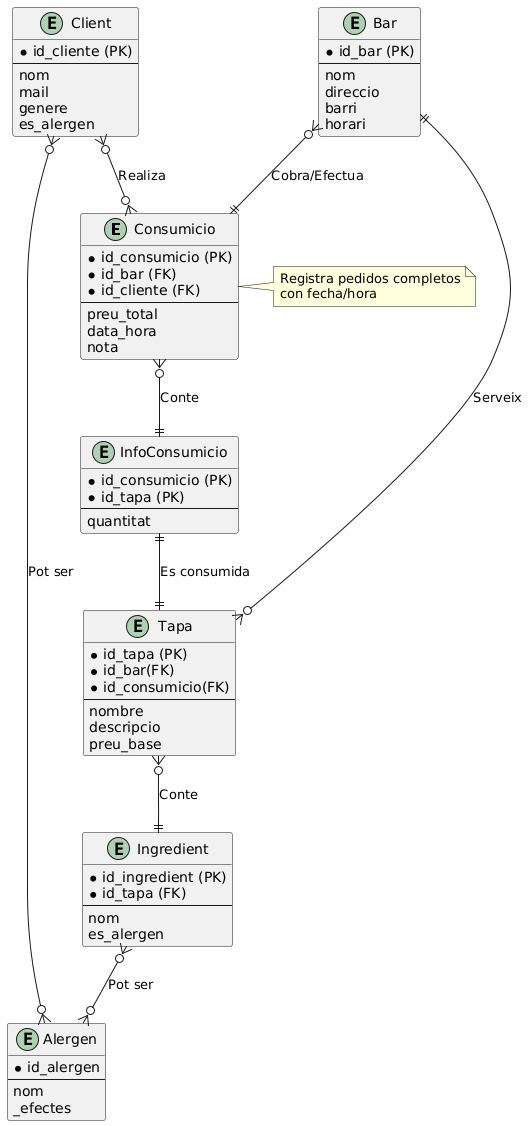
\includegraphics[width=0.65\linewidth]{E-R.png}
    \caption{Diagrama E-R generat amb PlantUML}
    \label{fig:plantuml-diagram}
\end{figure}


\newpage
\section{Recol·lecció i Neteja de Dades}

Per a alimentar la nostra base de dades de bars i tapes de Barcelona, hem seguit una metodologia estructurada que inclou diverses fonts de dades i un procés rigorós de neteja. Això ens ha permès garantir la qualitat i coherència de la informació recopilada.

\subsection{Fonts de Dades}

\noindent Les fonts de dades utilitzades en aquest projecte inclouen:

\begin{itemize}
    \item \textbf{Plataformes de Reviews (Scraping Inicial):}
    \begin{itemize}
        \item \textbf{TripAdvisor, TheFork, i Google Maps:} Es va extreure informació sobre els noms de bars, direccions, puntuacions i comentaris sobre tapes específiques (per exemple, \textit{"Les bombes d’aquest bar són espectaculars"}).
        \item \textbf{Eines:} Python, amb llibreries com \texttt{BeautifulSoup} o \texttt{Scrapy}, per realitzar el web scraping.
        \item \textbf{Desafiaments:} Identificar i estructurar dades no homogènies (exemple: formats diferents de puntuacions) i filtrar ressenyes falses mitjançant anàlisi de sentiment.
    \end{itemize}

    \item \textbf{Dades de Consum Propi (Manual):}
    \begin{itemize}
        \item \textbf{Registres personals del grup:} Arxius amb dades sobre consumicions pròpies, com les ressenyes detallades de tapes com les \textit{bombes} (\textit{"Bar X: Bombes 9/10 – crosta cruixent, farcit cremós"}).
        \item \textbf{Format:} Excel/CSV amb camps estructurats (nom\_bar, tapa, puntuació, data\_consumicio).
        \item \textbf{Enquestes a amics:} Recollida de dades mitjançant enquestes sobre hàbits de consum d’amics propers (exemple: \textit{"Quants cops has demanat braves aquest any?"}).
    \end{itemize}

    \item \textbf{Pàgines Web de Bars (Scraping):}
    \begin{itemize}
        \item \textbf{Menús online i webs de bars comuns:} Extracció d’informació sobre llistats de tapes, preus i ingredients (per exemple, \textit{Can Paixano, Quimet \& Quimet}).
        \item \textbf{Eines:} \texttt{Selenium} per a pàgines dinàmiques amb JavaScript.
    \end{itemize}

    \item \textbf{Xarxes Socials (Hashtags i Geolocalització):}
    \begin{itemize}
        \item \textbf{Instagram i TikTok:} Cercada de posts amb hashtags com \#TapasBarcelona, \#BombesBCN, o geolocalitzacions de bars.
        \item \textbf{Filtrat:} Anàlisi d’imatges i descripcions que mencionin tapes específiques.
    \end{itemize}
\end{itemize}

\subsection{Procés de Neteja de Dades}

Un cop recollides les dades, hem seguit els següents passos per garantir la seva qualitat i coherència:

\begin{itemize}
    \item \textbf{Estandarització de Formats:}
    \begin{itemize}
        \item Unificació de formats per a camps com preus (€4.50 → 4.50), dates (15/03/2025 → 2025-03-15), i barris (exemple: \textit{Gracia} → \textit{Gràcia}).
        \item \textbf{Eines:} Python amb \texttt{Pandas} i expressions regulars (Regex).
    \end{itemize}

    \item \textbf{Identificació de Duplicats:}
    \begin{itemize}
        \item Eliminació d'entrades duplicades de bars o tapes, com quan el mateix bar es repeteix en diferents fonts (exemple: TripAdvisor i Google Maps).
        \item \textbf{Tècnica:} Comparació de \texttt{nom\_bar} i \texttt{direccio} mitjançant fuzzy matching per a detectar errors tipogràfics.
    \end{itemize}

    \item \textbf{Gestió de Valors Faltants:}
    \begin{itemize}
        \item En cas de valors mancants (per exemple, el preu d'una tapa), es realitza una imputació mitjançant la mitjana dels preus d'altres tapes de la mateixa categoria (exemple: tapes \textit{braves} = €4-6).
        \item Si un bar no té horari, es marcarà com \textit{No disponible} per evitar inconsistències.
    \end{itemize}

    \item \textbf{Validació d’Al·lèrgens:}
    \begin{itemize}
        \item Creació d'un diccionari d’ingredients i al·lèrgens (per exemple, \textit{patata} → sense gluten) per a tapes amb etiquetatge poc clar.
        \item \textbf{Font Secundària:} Bases de dades públiques com FENIL per a validar ingredients comuns.
    \end{itemize}

    \item \textbf{Geocodificació:}
    \begin{itemize}
        \item Conversió d’adreces de bars a coordenades GPS (latitud, longitud) mitjançant l’API de Google Maps o OpenStreetMap.
    \end{itemize}
\end{itemize}

\subsection{Futur: Plataforma Col·laborativa}

En una fase posterior del projecte, es preveu/ ens agradaria implementar una plataforma on els usuaris puguin:

\begin{itemize}
    \item Afegir nous bars i tapes mitjançant formularis estandarditzats.
    \item Puntuar consumicions i verificar al·lèrgens.
    \item Corregir errors mitjançant un sistema de revisió comunitària.
\end{itemize}

Aquesta plataforma permetrà crear una base de dades rica, precisa i útil, tant per a amants de les tapes com per a persones amb restriccions alimentàries.
\section{Avanç de Consultes Mitjançant l'Àlgebra Relacional}

Gràcies a la base de dades dissenyada, podem realitzar diverses consultes per obtenir informació rellevant sobre els consumos realitzats als bars de Barcelona. A continuació es presenten alguns exemples de consultes que es podrien fer, utilitzant l'àlgebra relacional per expressar-les de manera formal.

\subsection{Consulta 1: Quin usuari ha consumit més en un bar?}

Per a realitzar aquesta consulta, necessitem identificar quin client (usuari) ha consumit més quantitat en un determinat bar. La consulta es basarà en la taula `Consumicio` per obtenir les quantitats consumides i l'usuari associat.

\textbf{Formula en àlgebra relacional}: 
Suposant que volem saber quin client ha consumit més en el bar amb l'`id\_bar = 1`:

\[
\text{Resultat} = \pi_{\text{id\_cliente}, \text{quantitat}} \left( \sigma_{\text{id\_bar} = 1} (\text{InfoConsumicio}) \bowtie \text{Consumicio} \right)
\]

Aquesta consulta filtra les consumicions per un determinat bar i després projecta els resultats en funció de l'`id\_cliente` i la `quantitat` consumida. Per trobar qui ha consumit més, caldria realitzar una agregació posterior.

\subsection{Consulta 2: Quin bar ha tingut més consumicions?}

Per a saber quin bar ha tingut més consumicions, podem realitzar una agregació de les comandes fetes a cada bar. Aquesta consulta farà ús de les taules `Consumicio` i `InfoConsumicio` per obtenir la informació relacionada amb els bars.

\textbf{Formula en àlgebra relacional}: 
Per obtenir el nombre de consumicions per a cada bar, fem:

\[
\text{Resultat} = \gamma_{\text{id\_bar}, \text{count}(\text{id\_consumicio})} (\text{Consumicio})
\]

Aquesta consulta retorna el nombre de consumicions per cada bar. Per a identificar el bar amb més consumicions.

\subsection{Consulta 3: Quin és l'ingredient més consumit?}

Per a saber quin és l'ingredient més consumit, necessitem fer una agregació de les quantitats de cada ingredient present a les consumicions. Aquesta consulta implicarà la taula `Ingredient` i `InfoConsumicio`, i caldria comptabilitzar quins ingredients apareixen més sovint.

\textbf{Formula en àlgebra relacional}: 
Per a trobar l'ingredient més consumit, podríem utilitzar la següent expressió:

\[
\text{Resultat} = \gamma_{\text{id\_ingredient}, \text{count}(\text{id\_tapa})} (\text{Ingredient} \bowtie \text{InfoConsumicio})
\]

Aquesta consulta fa una unió entre les taules `Ingredient` i `InfoConsumicio`, i després comptabilitza el nombre d'aparicions de cada ingredient. La resposta serà l'ingredient més freqüent.

\section{Conclusions}

En finalitzar aquesta primera fase del nostre projecte sobre el consum de tapes als locals barcelonins, hem establert una base sòlida per a la gestió i anàlisi de dades relacionades amb la gastronomia tradicional de la ciutat. Mitjançant el disseny d’un model Entitat-Relació detallat, hem definit les estructures necessàries per catalogar bars, tapes, ingredients i consumidors, així com les seves relacions.

Aquesta etapa inicial ens ha permès identificar les fonts de dades més rellevants —des de plataformes de reviews fins a registres personals— i establir un procés rigorós de neteja i estandardització per garantir la qualitat de la informació. A més, hem avançat en la definició d’àlgebra relacional per a consultes futures, com identificar els clients més freqüents, els bars amb més consum o els ingredients més populars.

El proper pas serà la implementació de la base de dades, que ens permetrà explotar aquesta informació per a:

\begin{itemize}
    \item Preservar la cultura gastronòmica local, donant visibilitat als bars autèntics i les seves tapes.
    \item Oferir eines útils per a persones amb restriccions alimentàries, com celíacs o vegetarians.
    \item Analitzar patrons de consum (preferències per barris, horaris o estacionalitat) i tendències emergents.
\end{itemize}

El nostre objectiu final és que aquesta base de dades no només serveixi com a arxiu de la tradició culinària barcelonina, sinó també com a recurs per a consumidors i professionals del sector, fomentant decisions informades i contribuint a la sostenibilitat dels bars tradicionals en un context de canvis gastronòmics globals.

Amb aquests fonaments, estem preparats per avançar cap a la construcció d’un sistema funcional i escalable, que reflecteixi la riquesa de les tapes com a element identitari de Barcelona.
\subsection{Aportacions:}
El desenvolupament d'aquest projecte sobre el consum de tapes a Barcelona ha estat possible gràcies a les contribucions específiques de cada membre de l'equip:

\begin{itemize}
\item \textbf{Pau Queralt Muñoz}: S'ha encarregat de la redacció principal del document, participant activament en el disseny del model Entitat-Relació i en l'estructuració global del projecte.
\item \textbf{Alberto Moreno Martinez}: Ha liderat la recollida inicial de dades, a més de contribuir significativament en la redacció dels continguts i en la ideació dels objectius del projecte.

\item \textbf{Gerard Fideu Garcia}: Com a redactor secundari, ha participat en l'elaboració dels continguts i ha estat responsable del disseny i programació del diagrama UML que representa el model conceptual.
\end{itemize}

Aquest treball col·laboratiu ha permès crear una base sòlida per a l'anàlisi dels hàbits de consum de tapes a Barcelona, amb un model ben definit que permetrà futures ampliacions. Els pròxims passos se centraran en la implementació pràctica de la base de dades i en l'anàlisi i neteja de les dades recollides.

\section{Anexos}

\subsection{Repositori GitHub}

Tots els arxius del projecte, incloent-hi el codi font del model Entitat-Relació, les dades recopilades i altres elements relacionats, es poden trobar al nostre repositori de GitHub. A continuació, proporcionem l'enllaç per accedir-hi:

\url{https://github.com/Pantanosso/BDProjectBombas}

Aquest repositori conté:
\begin{itemize}
    \item El codi complet del model Entitat-Relació generat.
    \item Dades recopilades durant la fase inicial del projecte.
    \item Scripts i eines utilitzades per a la neteja i anàlisi de les dades.
    \item Documentació relacionada amb la implementació de la base de dades.
\end{itemize}

\end{document}

